%=========================================================

% Here you can choose to compile with or without solutions.
% However, this definition is ignored if you use any
% command from the `Makefile`.
\providecommand{\withSol}{\iftrue}

%=========================================================

\documentclass
[twoside,english,colorbacktitle,accentcolor=tud9c]
{tudexercise}

\usepackage[T1]{fontenc}
\usepackage[latin9]{inputenc}
\usepackage{amstext}
\usepackage{float}
\usepackage{amsmath}
\usepackage{graphicx}
\usepackage{setspace}
\usepackage{multicol}
\usepackage{mathtools}
\usepackage{dsfont}
\usepackage{units}
\usepackage{subfigure}
\usepackage{color}
\usepackage{booktabs}
\usepackage{fancyref}
\usepackage[ngerman,english]{babel}
\usepackage{listings}

%=========================================================
% Configuration for code display

\definecolor{dkgreen}{rgb}{0,0.6,0}
\definecolor{gray}{rgb}{0.5,0.5,0.5}
\definecolor{mauve}{rgb}{0.58,0,0.82}

\lstset{frame=tb,
	language=Python,
	aboveskip=3mm,
	belowskip=3mm,
	showstringspaces=false,
	columns=flexible,
	basicstyle={\small\ttfamily},
	numbers=none,
	numberstyle=\tiny\color{gray},
	keywordstyle=\color{blue},
	commentstyle=\color{dkgreen},
	stringstyle=\color{mauve},
	breaklines=true,
	breakatwhitespace=true,
	tabsize=4
}
%=========================================================

\def\homework{3}
\def\homeworkVer{1}
\def\homeworkSolVer{1}
\def\lecture{Machine Learning}
\def\semester{Summer Semester 2019}
\def\prof{Prof. Dr. J. Peters, H. Abdulsamad, S. Stark, D.Koert}
\def\deadline{Due date: Friday, 5 Juli 2019 (17:00)\\
You need to hand in the pdf in moodle \textbf{and} a printed version to the postbox from the IAS secretary office (S2 02 | E315)}

%=========================================================

\ifcsname withSol\endcsname\else
  \expandafter\let\csname withSol\expandafter\endcsname
                  \csname iffalse\endcsname
\fi

\withSol
	\usepackage[solutions]{iasHomework}
\else
	\usepackage{iasHomework}
\fi

%=========================================================

% USE YOUR NAMES!
\newcommand{\studentdata}{Peter Nickl, 1941346 \qquad Steffen Sch�fer, 2635897}
%\newcommand{\studentdata}{John Doe, 1234567 \qquad Jane Doe, 7654321}

\begin{document}
	
	\hwtitle{}
	\maketitle
	
	\begin{examheader}
		\normalsize
		\vspace{-1em}
		Name, Surname, ID Number \hfill \studentdata{}
		\vspace{-1em}
	\end{examheader} 
	\textbf{Group ID : 146}\\
	\textbf{Name, Surname, ID Number \hfill \studentdata{}}

	\newif\ifvimbug
\vimbugfalse

\ifvimbug
\begin{document}
\fi

\exercise{Linear Regression}

In this exercise, you will use the dataset \texttt{linRegData.txt}, containing $150$ points in the format \texttt{<input variable, output variable>}. The input is generated by a sinusoid function, while the output is the joint trajectory of a compliant robotic arm. 
The first 20 data points are the training set and the remainder are the testing set.

\begin{questions}

%----------------------------------------------

\begin{question}{Polynomial Features}{10}
Write the equation of the model and fit it with polynomial features. Using the Root Mean Square Error (RMSE) as a metric for the evaluation, select the complexity of the model (up to a 21st degree polynomial) by evaluating its performance on the testing data. Which is the best RMSE you achieve and what is the model complexity? Does it change if we evaluate our model on the training data? Comment your findings and plot the RMSE for each case (use two lines, one for evaluation on training data, one for evaluation on testing data).
For the estimation of the optimal parameters use a ridge coefficient of $\lambda=10^{-6}$.
\\Using what you think is the best learned model from the previous point, show in a single plot the ground truth (full dataset) and the model prediction over it.
Attach snippets of your code showing how you generate polynomial features and how you fit the model.

\begin{answer}\end{answer}

\end{question}

%----------------------------------------------

\begin{question}{Gaussian Features}{4}
Now use Gaussian features. Each feature is a Gaussian distribution were the means are distributed linearly in $x \in[0,2]$ and the variance is set to $\sigma^2=0.02$. The features have to be normalized, i.e., they have to sum to one at every $x$. Using 10 features generate a plot with the activation of each feature over time (i.e., plot the matrix $\Phi$). Attach a snippet of your code showing how to compute Gaussian features.

\begin{answer}\end{answer}

\end{question}

%----------------------------------------------

\begin{question}{Gaussian Features, Continued}{4}
Repeat the process of fitting the model using the Gaussian features from the previous question. Compare the RMSE on the testing data using $15 \ldots 40$ basis functions and plot the RMSE. Which number of basis functions has the best performance and what is the best RMSE? Use a ridge coefficient of $\lambda=10^{-6}$.

\begin{answer}\end{answer}

\end{question}

%----------------------------------------------

\begin{question}{Bayesian Linear Regression}{10}
Using Bayesian linear regression, plot the mean and the standard deviation of the predictive distribution learned using the first $\{10, 12, 16, 20, 50, 150\}$ data points (one plot per case; plot it in the interval $x\in[0,2]$).
Discuss how the model uncertainty changes with the amount of data points and the problem of overfitting with Bayesian linear regression.
Use the best performing polynomial features that you found in 3.1a, a ridge coefficient of $\lambda=10^{-6}$, and assume Gaussian noise with $\sigma^2=0.0025$. 

\begin{answer}\end{answer}
\end{question}

%----------------------------------------------

\begin{question}[bonus]{Cross Validation}{5}
So far, we have split our dataset in two sets: training data and testing data. Cross-validation is a more sophisticated approach for model selection. Discuss it and its variants, pointing out their pro and cons.
\end{question}

\begin{answer}\end{answer}

\end{questions}

	
	\newif\ifvimbug
\vimbugfalse

\ifvimbug
\begin{document}
\fi

\exercise{Linear Classification}

In this exercise, you will use the dataset \texttt{ldaData.txt}, containing 137 feature points $\vec x$. The first 50 points belong to class $C_1$, the second 43 to class $C_2$, the last 44 to class $C_3$.


\begin{questions}
%----------------------------------------------

\begin{question}{Discriminative and Generative Models}{4}
Explain the difference between discriminative and generative models and give an example for each case.
Which model category is generally easier to learn and why?
 
\begin{answer}
\textbf{Generative models} first use the underlying data to deduce properties of the underlying probability distribution in form of the class-doncitional densties $p(x|C_k)$ for each class $C_k$. Seperatly they infer the prior class probabilities $p(C_k)$. After that, they use Bayes'theorem  in the form 
\begin{equation}
	\frac{p(x|C_k) p(C_k)}{p(x)}
\end{equation}
to fint the posteriori class probabilities $p(C_k|x)$. Now decision theory is used to determine class membership. 

Since in theory we can use these distribution to create new data, this is called a gernative model. Also note that generative models also work when modeling the joint distribution $p(x, C_k)$ and normalizing. 


\textbf{Discriminative models} determine the posterior class probabilities $p(C_k|x)$ directly. After that decision theory is used to each new input to a class. 


Because generative models need the joint distribution $p(x,C_k)$ for calculating the posterior distribution, instead of deriving it directly, they're much harder to train. This is especially true if $x$ is highly dimensional, since then we need a very big dataset to model class-doncitional densities correctly.

 

\end{answer}

\end{question}

%----------------------------------------------

\begin{question}{Linear Discriminant Analysis}{12}
Use Linear Discriminant Analysis to classify the points in the dataset, i.e., assume Gaussian distributions in each class with equal covariances and use the posterior distributions for assigning classes. Attach two plots with the data points using a different color for each class: one plot with the original dataset, one with the samples classified according to your LDA classifier. Attach a snippet of your code and discuss the results. How many samples are misclassified? (You are allowed to use built-in functions for computing the mean and the covariance.)

\begin{answer}\end{answer}
\end{question}

%----------------------------------------------

\end{questions}

	
	\newif\ifvimbug
\vimbugfalse

\ifvimbug
\begin{document}
\fi

\exercise{Principal Component Analysis}
In this exercise, you will use the dataset \texttt{iris.txt}. It contains data from three kind of Iris flowers (`Setosa', `Versicolour' and `Virginica') with 4 attributes: sepal length, sepal width, petal length, and petal width. Each row contains a sample while the last attribute is the label ($0$ means that the sample comes from a `Setosa' plant, $1$ from a `Versicolour' and $2$ from `Virginica').
(You are allowed to use built-in functions for computing the mean, the covariance, eigenvalues and eigenvectors.)

\begin{questions}

%----------------------------------------------

\begin{question}{Data Normalization}{3}
Normalizing the data is a common practice in machine learning. Normalize the provided dataset such that it has zero mean and unit variance per dimension. Why is normalizing important?
Attach a snippet of your code. 

\begin{answer}
In machine learning some methods like PCA take the variance of the features as a criterion for dimensionality reduction. If the feature differ in their range, the means and the variances of the features will have a different scale. To achieve better comparability among the features it is common to normalize the data to unit variance and zero mean. The normalization can be achieved by applying the following formula to all datapoints $x_i$ for each feature separately:
\begin{equation*}
\frac{x_i-mean_{feature}}{standard\_deviation_{feature}}
\end{equation*}
We calculated the means of the features as follows:
$$means=\begin{bmatrix} 
5.84333333 & 3.054 & 3.75866667 &1.19866667
\end{bmatrix}$$
We calculated the standard deviation of the features as follows:
$$standard\_deviation=\begin{bmatrix} 
0.82530129 & 0.43214658 & 1.75852918 & 0.76061262
\end{bmatrix}$$
We apply the normalization to the dataset according to the following code snippet.\\
\lstinputlisting[language=Python]{code/PCA_normalize.py}
\end{answer}

\end{question}

%----------------------------------------------

\begin{question}{Principal Component Analysis}{8}
Apply PCA on your normalized dataset and generate a plot showing the proportion (percentage) of the cumulative variance explained. 
How many components do you need in order to explain at least $95\%$ of the dataset variance? 
Attach a snippet of your code.
\begin{answer}
For doing the PCA, after normalizing, we have to compute the covariance matrix and subsequently calculate the eigenvectors and eigenvalues of the covariance matrix.\\
As Figure \ref{fig:1} shows, by using two principal components we can explain 95,8\% of the cumulative variance. The four bars are calculated by using the following formula, whereas the eigenvalues are sorted from the biggest eigenvalue to the smallest eigenvalues:
\begin{equation*}
\textrm{proportion of cumulative variance explained by n biggest eigenvectors} = \frac{\textrm{sum of n biggest eigenvalues}} {\textrm{sum of all eigenvalues}} 
\end{equation*}
For the covariance matrix of the normalized data we obtain:
$$\Sigma=\begin{bmatrix} 
1.00671141 & -0.11010327 & 0.87760486 & 0.82344326 \\
-0.11010327 & 1.00671141& -0.42333835& -0.358937  \\
0.87760486 &-0.42333835 & 1.00671141 & 0.96921855 \\
0.82344326& -0.358937  &  0.96921855 & 1.00671141
\end{bmatrix}$$
The eigenvalues have the following values:
$$eigenvalues = \begin{bmatrix} 
2.93035378 & 0.92740362& 0.14834223 &0.02074601
\end{bmatrix}$$
The eigenvectors have the following values. The eigenvectors are sorted according to their respective eigenvalues above. Each column contains one eigenvector.
$$eigenvectors = \begin{bmatrix} 
 0.52237162 &-0.37231836 &-0.72101681 & 0.26199559\\
 -0.26335492 &-0.92555649 & 0.24203288 &-0.12413481\\
 0.58125401 &-0.02109478&  0.14089226 &-0.80115427\\
 0.56561105& -0.06541577 & 0.6338014 &  0.52354627
\end{bmatrix}$$
The following code snippet shows the code for doing the PCA and for plotting.\\
\lstinputlisting[language=Python]{code/PCA_explained_variance.py}
\end{answer}
\begin{figure}[h!]
	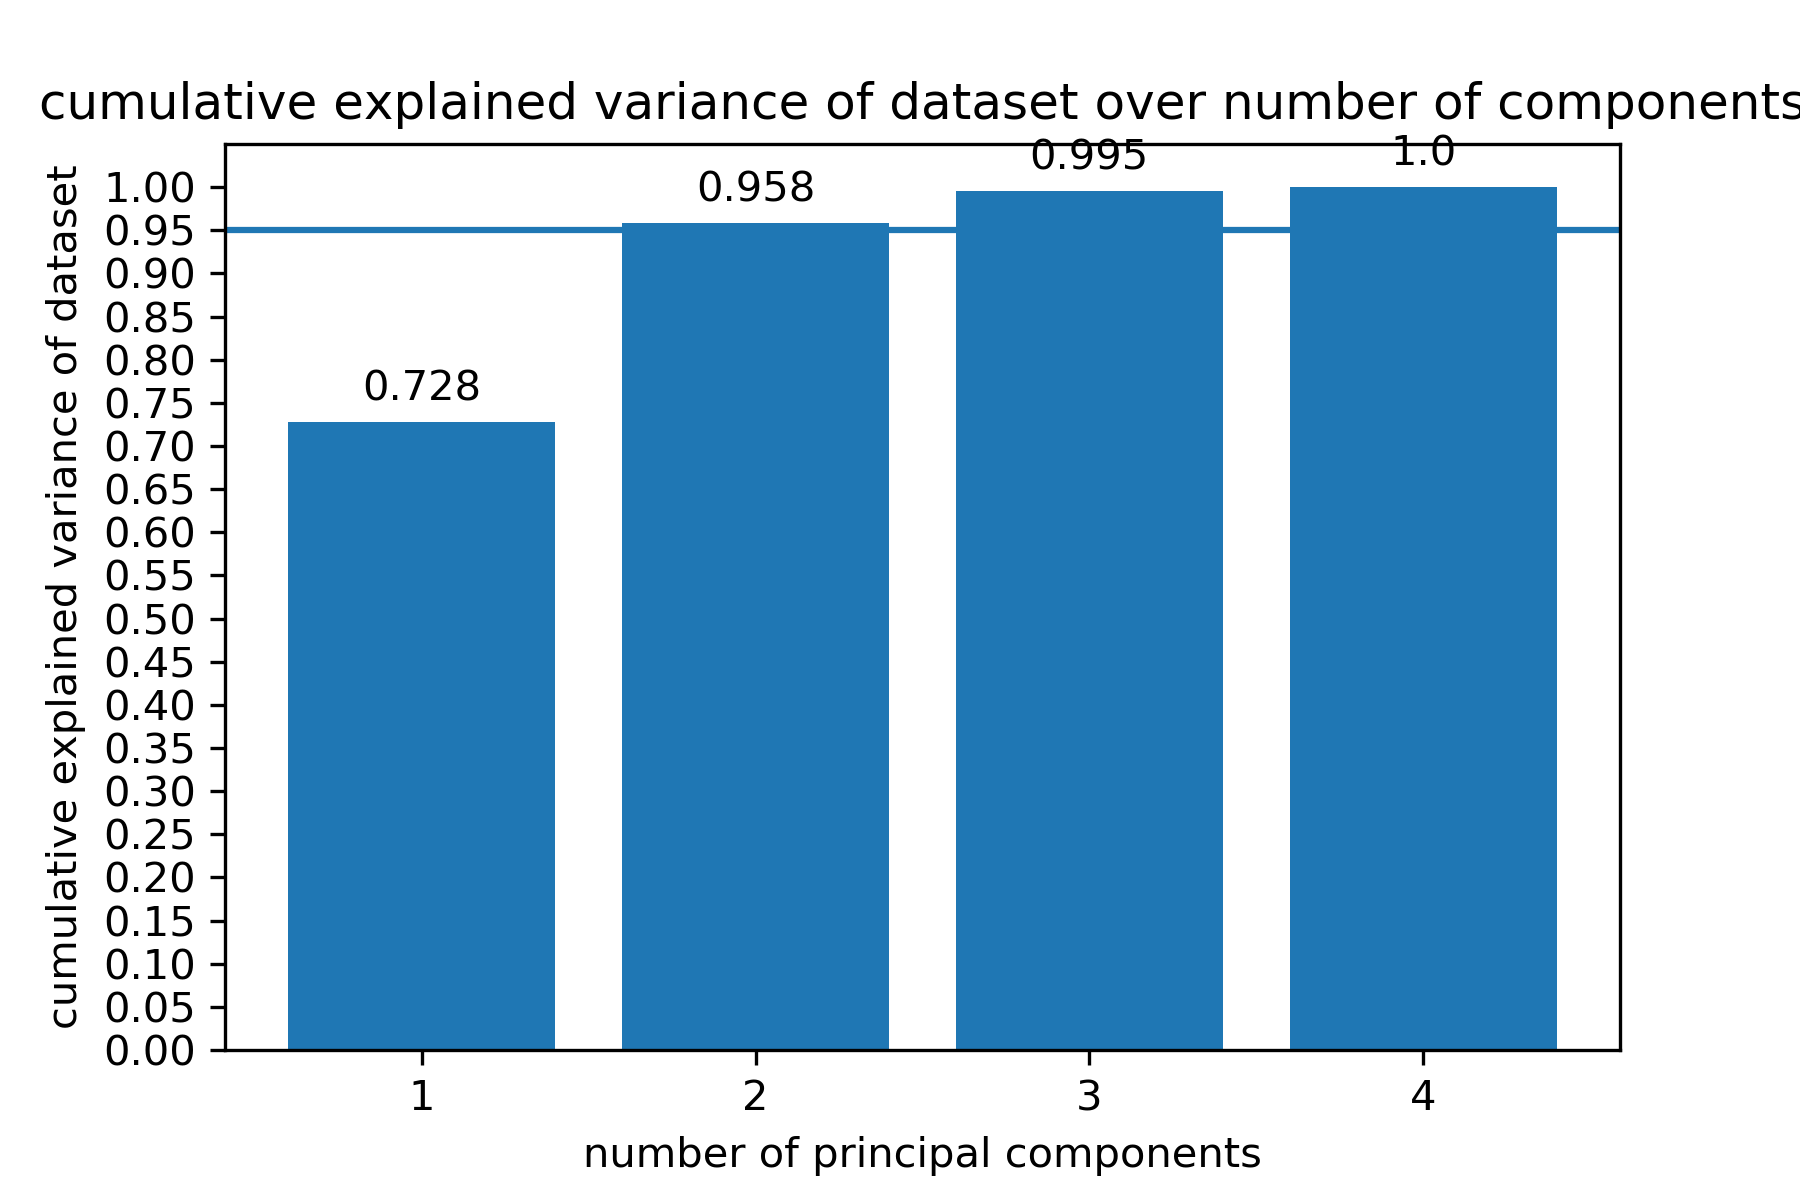
\includegraphics[width=0.8\linewidth]{pictures/explained_var_cumulative.png}
	\centering
	\caption{Cumulative explained variance of dataset over number of principal components.}
	\label{fig:1}
\end{figure}
\end{question}

%----------------------------------------------

\begin{question}{Low Dimensional Space}{6}
Using as many components as needed to explain $95\%$ of the dataset variance, generate a scatter plot of the lower-dimensional projection of the data. Use different colors or symbols for data points from different classes. 
What do you observe? Attach a snippet of your code.
\begin{answer}
For projecting the data to the lower dimensional space we use the following formula on the normalized dataset:
\begin{equation}
\mathbf{a}^{n}=\mathbf{B}^{\top}\mathbf{x}^{n}
\end{equation}
$\mathbf{a}^{n}$ is the projected data, $\mathbf{B}$ is a matrix containing the eigenvectors - in our case the two eigenvectors corresponding to the two biggest eigenvalues, for obtaining 2-dimensional projection - and $\mathbf{x}^{n}$ is the projected data. The two biggest eigenvalues with corresponding eigenvectors are:
$$eigenvalues =\begin{bmatrix} 
2.93035378 & 0.92740362
\end{bmatrix}$$
The eigenvectors have the following values. The eigenvectors are sorted according to their respective eigenvalues above. Each column contains one eigenvector.
$$eigenvectors = \begin{bmatrix} 
 0.52237162 &-0.37231836 \\
 -0.26335492 &-0.92555649 \\
 0.58125401 &-0.02109478\\
 0.56561105& -0.06541577 
\end{bmatrix}$$
The 2-dimensional projection leads to the scatter plot in Figure \ref{fig:2}. \\
We can observe that the Versicolour class is clearly separated from the Setosa and Verginica classes in the two-dimensional space. Between the Setoas and the Viriginica class, there is some overlapping, but the class means and variances are still different from each other. Since the two-dimensional projection contains over 95\% of the variance of the unprojected dataset, these results can be transferred to the unprojected dataset, too.\\
Building upon the previously used code, we have used the following code for the two-dimensional projection and the scatter plot.\\
\lstinputlisting[language=Python]{code/PCA_scatter.py}
\end{answer}
\begin{figure}[h!]
	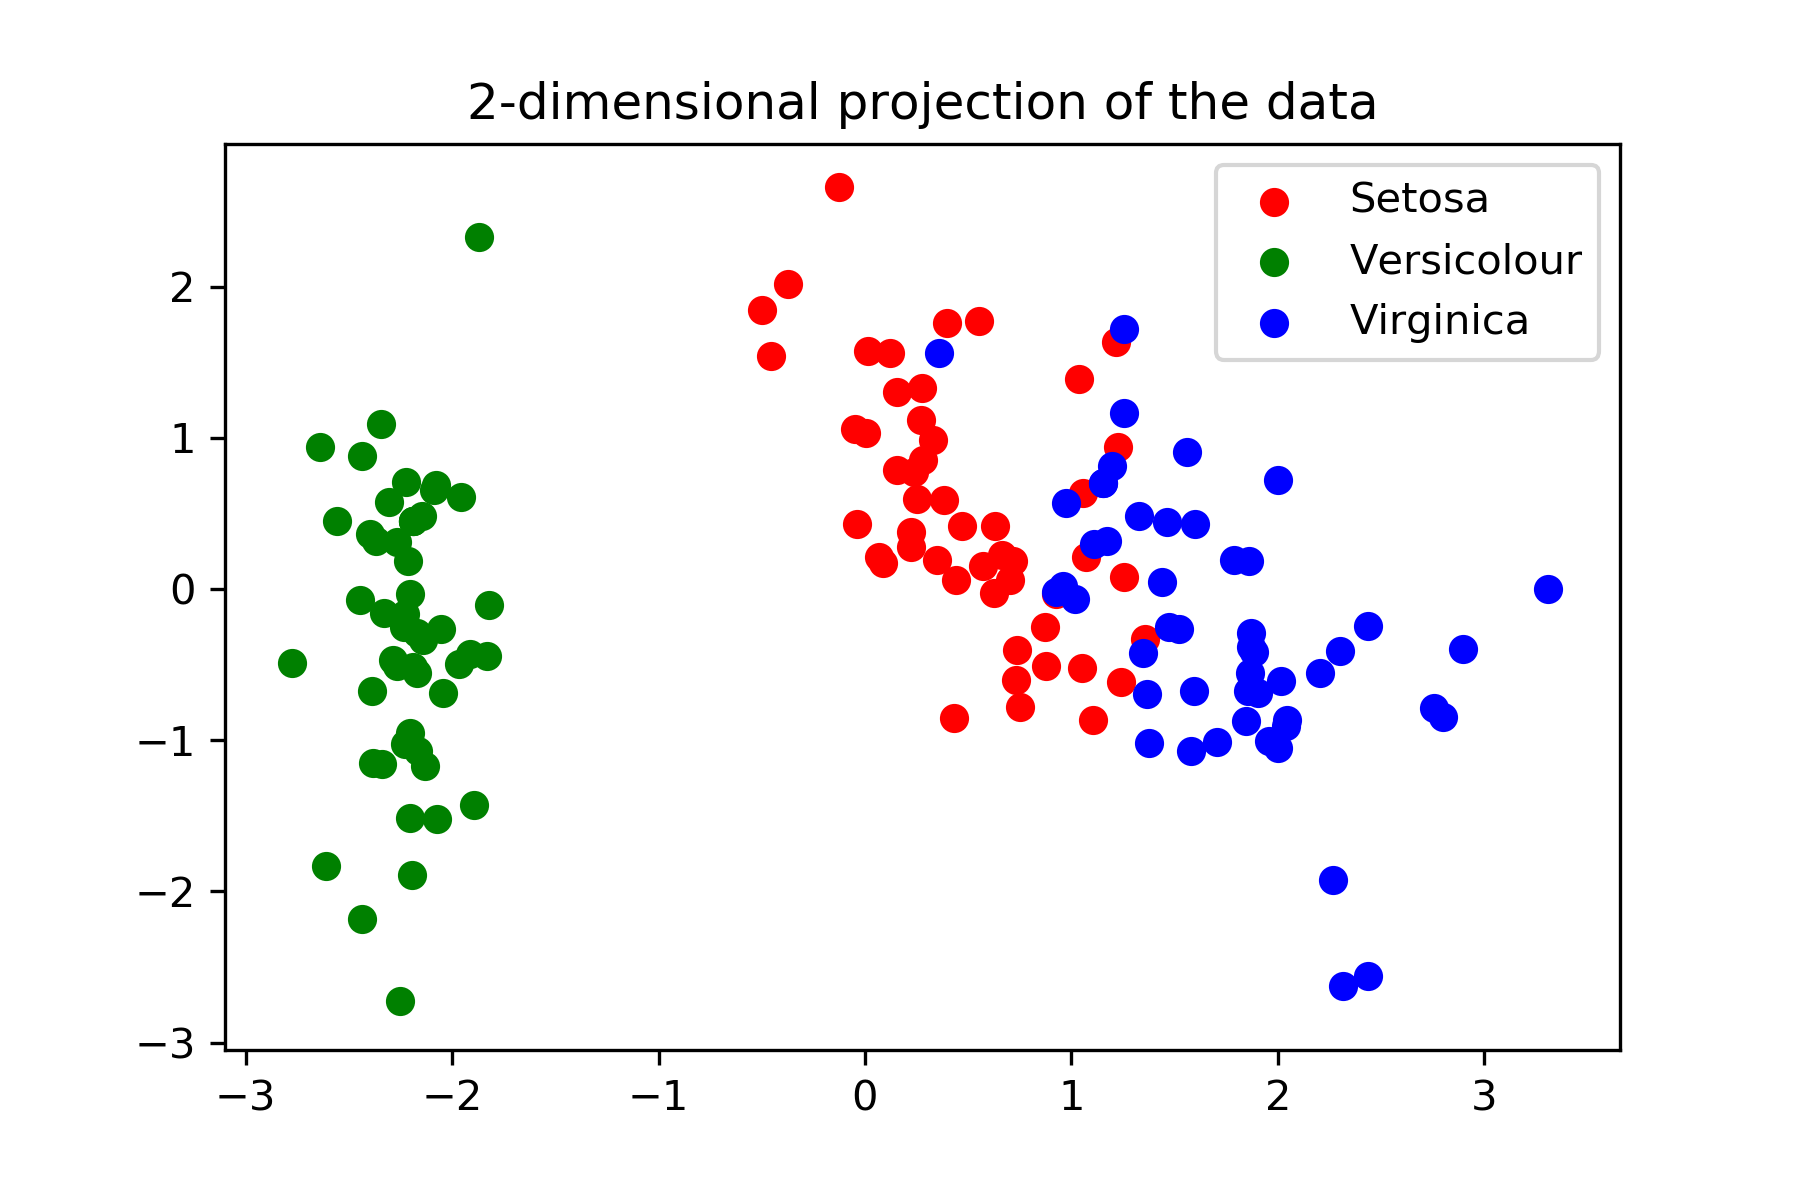
\includegraphics[width=0.8\linewidth]{pictures/PCA_scatter.png}
	\centering
	\caption{Scatter plot of the 2-dimensional projection of the data.}
	\label{fig:2}
\end{figure}
\end{question}

%----------------------------------------------

\begin{question}{Projection to the Original Space}{6}
Reconstruct the original dataset by using different number of principal components. Using the normalized root mean square error (NRMSE) as a metric, fill the table below (error per input versus the amount of principal components used).

\begin{tabular}{c|r|r|r|r}
N. of components & $x_1$ & $x_2$ & $x_3$ & $x_4$ \\
\hline
1 & & & & \\
2 & & & & \\
3 & & & & \\
4 & & & &
\end{tabular}

Attach a snippet of your code.
(Remember that in the first step you normalized the data.)

\begin{answer}
For reconstructing the data, we use the following formula:
\begin{equation*}
\tilde{\mathbf{x}}^{n}=(\mathbf{B a}^{n} \cdot standard\_deviation_{feature})+ mean_{feature}
\end{equation*}
$\mathbf{B}$ contains as many eigenvectors as principal components we use for reconstructing the dataset. $\mathbf{a}^{n}$ is the lower dimensional projection of the data. We also need the standard deviation and mean of each feature, in order to undo the normalization step.\\
We then compute the $NRMSE$ for every feature as follows:
\begin{equation*}
NRMSE = \frac{RMSE}{x_{max}-x_{min}}
\end{equation*}
$x_{max}$ and $x_{min}$ are the minimal and maximal values of the respective features. The $RMSE$ is calculated as follows:
\begin{equation*}
\mathrm{RMSE}=\sqrt{\frac{\sum_{n=1}^{N}(\tilde{x}_{n}-x_{n})^{2}}{N}}
\end{equation*}
$\tilde{x}_{n}$ are the reconstructed values of the features and $x_{n}$ are the values from the original dataset.
By this we can fill in the table as follows:\\

\begin{tabular}{c|r|r|r|r}
N. of components & $x_1$ & $x_2$ & $x_3$ & $x_4$ \\
\hline
1 & 0.10397936 &0.16086196& 0.03835783 &0.08311765 \\
2 & 0.06403369 &0.0170341  &0.03788015 &0.08070068\\
3 & 0.00862221& 0.00320869 &0.03427903 &0.02381893\\
4 & 7.80185215e-17& 8.17102022e-17 &9.95720008e-17 &6.11515656e-17 
\end{tabular}\\ \\ \\
It can be noted, that the NRMSE is extremely small, but not zero, when all four components are used to reconstruct the data. This is due to numerical inaccuray. Building upon the previously show code, this is the code we used for the projection to the original space and the calculation on the NRMSE:\\
\lstinputlisting[language=Python]{code/PCA_original.py}
\end{answer}
\end{question}

\begin{question}[bonus]{Kernel PCA}{5}
Throughout this class we have seen that PCA is an easy and efficient way to reduce the dimensionality of some data. However, it is able to detect only linear dependences among data points. A more sophisticated extension to PCA, \emph{Kernel PCA}, is able to overcome this limitation. 
This question asks you to deepen this topic by conducting some research by yourself: explain what Kernel PCA is, how it works and what are its main limitations. Be as concise (but clear) as possible.

\begin{answer}\end{answer}
\end{question}

\end{questions}


\end{document}